\documentclass[12pt]{article}
\usepackage{amsmath}
\usepackage{graphicx}
\usepackage{hyperref}
\usepackage{geometry}
\geometry{margin=1in}


\title {HW6 Report: Classification Model Comparison}
\author{Thomas Meltesen}
\date{\today}

\begin{document}

\maketitle

\section{Goal}
Presents the process and results of comparing multiple classification models on a given dataset. The workflow includes loading and preprocessing the data, training and evaluating classifiers, ranking their performance, and drawing conclusions based on the results.

\section{The Dataset}
\begin{itemize}
    \item The data set used is a 13 feature (X1 - X13) all on varying scales to classify classes 0,1, and 2.
    \item The data was imported using pandas read csv function.
    \item The class distribution for the data set is shown below a total of 178 samples was used from this data set.
    % Class Distribution Table
\begin{table}[h!]
\centering

\begin{tabular}{lc}
\hline
Class    & Count \\
\hline
class\_1 & 71    \\
class\_0 & 59    \\
class\_2 & 48    \\
\hline
\end{tabular}
\caption{Class Distribution in the Dataset}
\end{table}
\end{itemize}

\section{Pre-proccessing}
\begin{itemize}
    \item Due to the low sample count, the data set was stratified to allow for appropriate class distributions across splits. With that, it was split 75-25 development and test to allow for accurate representation for both splits. Similarly, the random state was set to 42 for reproducibility across runs. The resulting tables for development and test class distribution is shown below.

    \begin{table}[h!]
\centering

\begin{tabular}{lc}
\hline
Class & Count \\
\hline
1     & 53    \\
0     & 44    \\
2     & 36    \\
\hline
\end{tabular}
\caption{Class Distribution in Development Set}
\end{table}

\begin{table}[h!]
\centering

\begin{tabular}{lc}
\hline
Class & Count \\
\hline
1     & 18    \\
0     & 15    \\
2     & 12    \\
\hline
\end{tabular}
\caption{Class Distribution in Test Set}
\end{table}

    \item After the data was split and stratified, it was then Standard Scaled, fitted and transformed on the development set and transformed the test set to allow for appropriate value ranges. Similarly, the Y variables were Label Encoded since ML models can't take in string inputs.
\end{itemize}

\section{Ranking the Classifiers}
\begin{itemize}
    \item The classifiers that were compared are: Logistic Regression, LDA, QDA.
    \item I ran a 5-fold stratified cross validation on each classifier. Each is scored on the f1 weighted metric. Since this data set is imbalanced with class distributions inherently from the data set and it is multiclass (i.e. K\texttt{>}2). The CV scores for the f1 weighted are shown below along with the mean.
    % Cross-validation Scores Table
\begin{table}[h!]
\centering

\begin{tabular}{lcc}
\hline
Classifier           & CV Scores & Mean CV Score ($\pm$ 2 std) \\
\hline
Logistic Regression  & 0.8875, 0.8879, 0.8535, 0.8089, 0.9618 & 0.8799 ($\pm$ 0.1002) \\
LDA                  & 0.8875, 0.8117, 0.8180, 0.8840, 0.9216 & 0.8646 ($\pm$ 0.0854) \\
QDA                  & 0.7778, 0.6947, 0.6246, 0.7682, 0.8072 & 0.7345 ($\pm$ 0.1325) \\
\hline
\end{tabular}
\caption{Cross-validation Scores for Each Classifier}
\end{table}
\item Based on the model ranking below and the CV scores found above, I'd ultimately choose logistic regression as the best performing model in this scenario due to it's CV scores. But moving on I need to see how it would perform in later classifications on the test set.
% Model Rankings Table
\begin{table}[h!]
\centering

\begin{tabular}{clc}
\hline
Rank & Classifier           & Mean CV Score \\
\hline
1    & Logistic Regression  & 0.8799 \\
2    & LDA                  & 0.8646 \\
3    & QDA                  & 0.7345 \\
\hline
\end{tabular}
\caption{Model Rankings Based on Mean CV Score}
\end{table}
    
\end{itemize}

\section{Training / Assessing Performance}
\begin{itemize}
    \item When training and testing each classifier I first analyzed it's accuracy for both the train and test as shown below.

% Train and Test Accuracy Table
\begin{table}[h!]
\centering

\begin{tabular}{lcc}
\hline
Classifier           & Train Accuracy & Test Accuracy \\
\hline
LDA                  & 0.9023         & 0.8667        \\
QDA                  & 0.9624         & 0.8222        \\
Logistic Regression  & 0.9323         & 0.8444        \\
\hline
\end{tabular}
\caption{Train and Test Accuracy for Each Classifier}
\end{table}
    \item Compared to the previous section with Logistic Regression being the highest ranked model there was a discrepancy with what I found training and assessing the performance of these 3 models. LDA seems to allow for an overall higher test accuracy than logistic regression. Which could be an identifier to something either not being done in training like hyper parameter optimization. Also, If class covariance matrices are roughly equal, LDA often performs similarly or better because it estimates class means + shared covariance and uses assumptions. Logistic regression is discriminative. On small datasets, LDA can sometimes outperform discriminative ones because they estimate fewer parameters under assumptions. Which ultimately leads to the conclusion that there could just be not enough representative samples for our data set to give an accurate show of model performance.
\maketitle

\begin{figure}[h!]
    \centering
    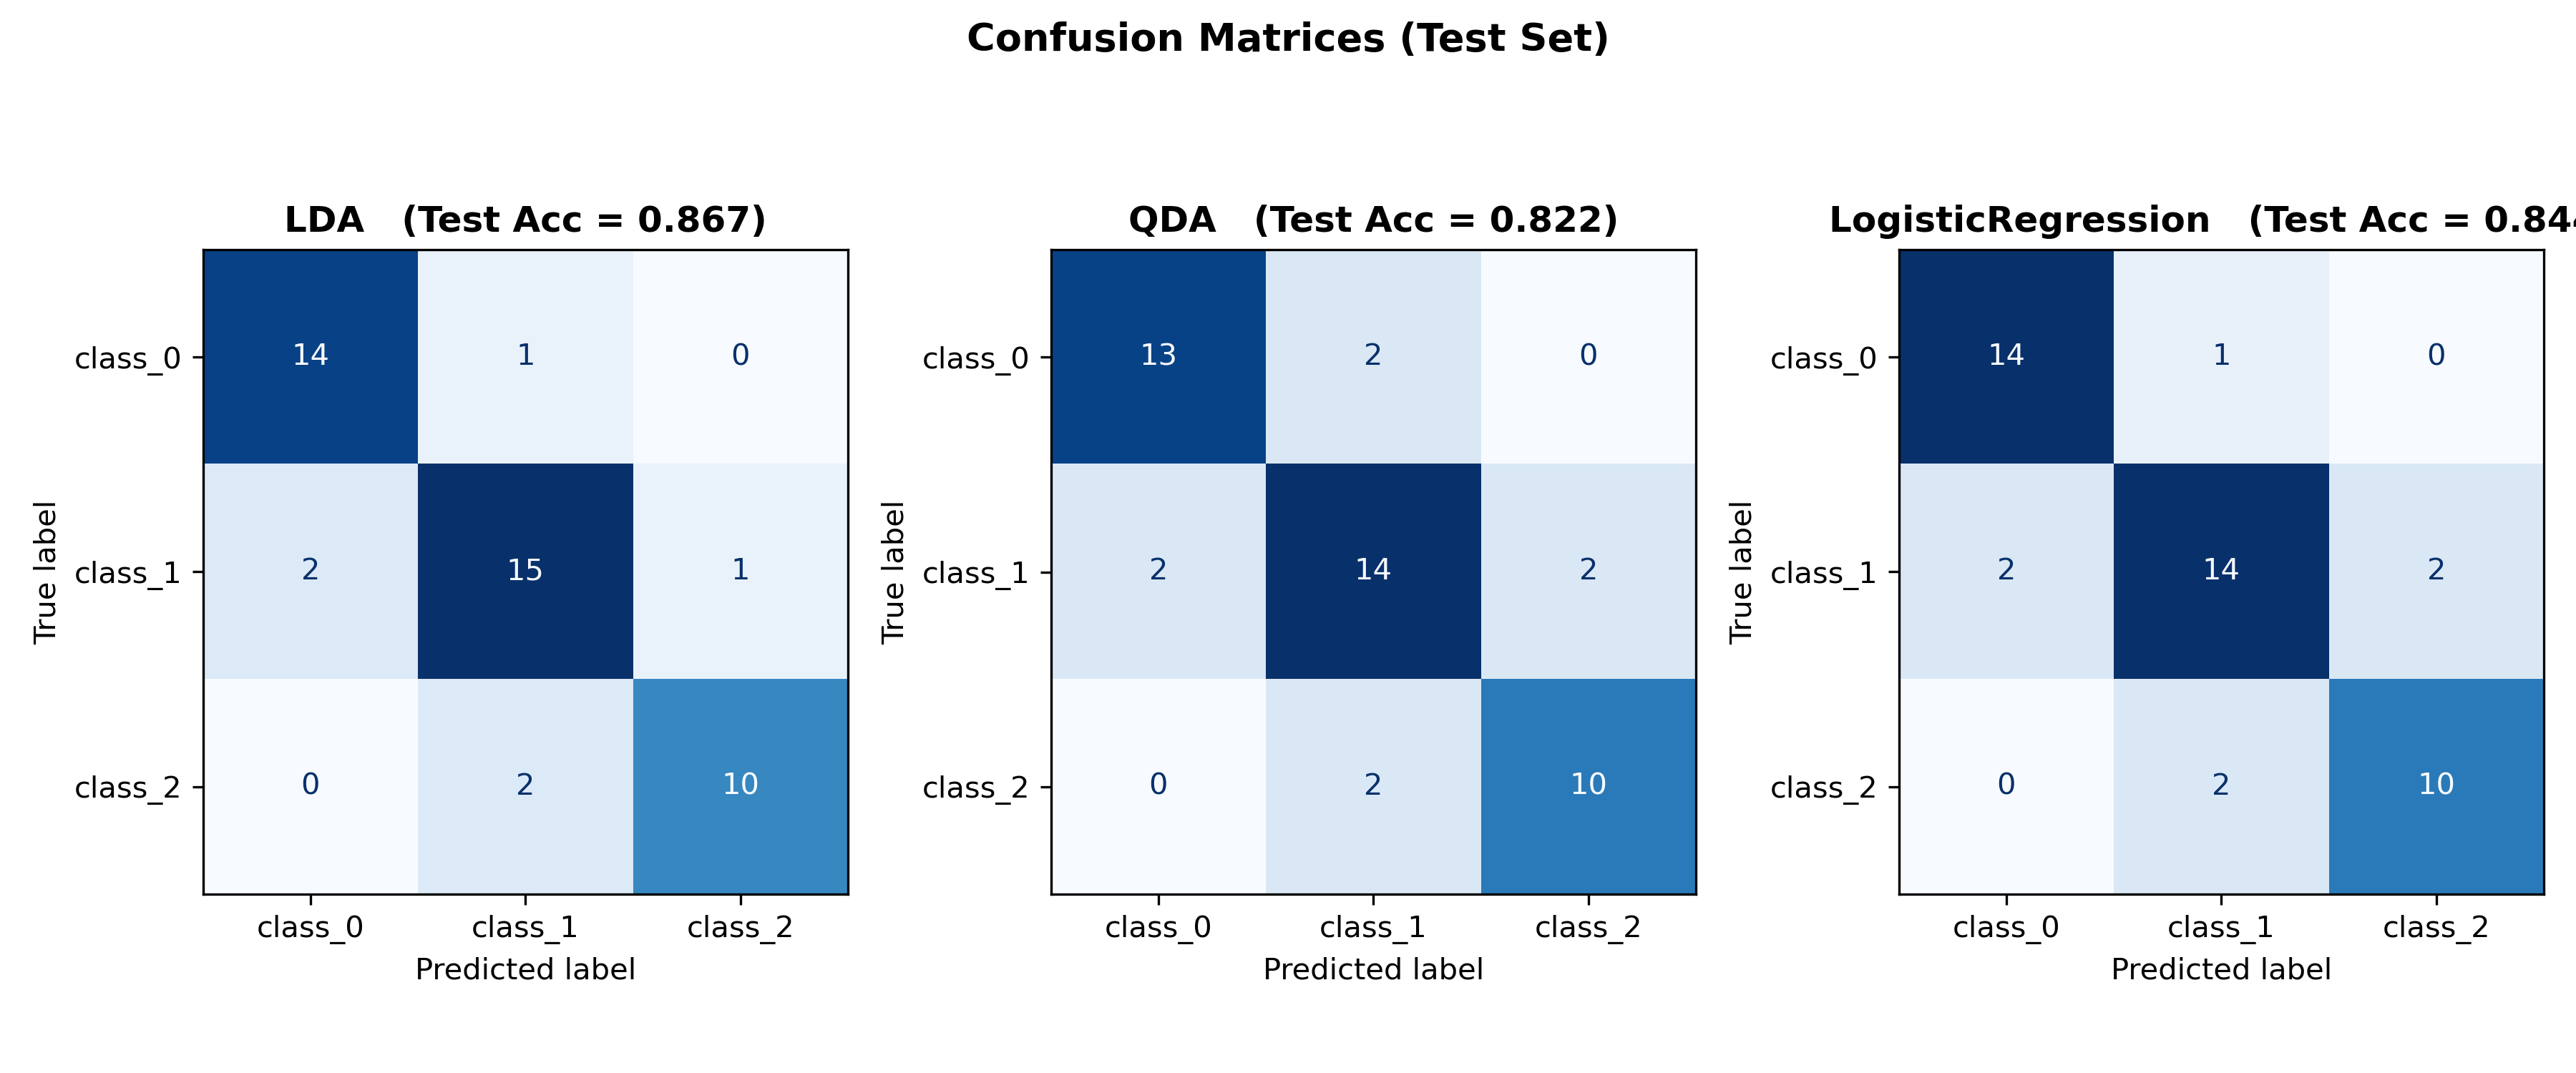
\includegraphics[width=0.9\textwidth]{confusion_matrices.png}
    \caption{Confusion matrices for LDA, QDA, and Logistic Regression on the test set.}
    \label{fig:confusion_matrices}
\end{figure}
    \item The classification reports and confusion matrices for each classifier back this assumption. Given, we do have an imbalance between our samples, gives LDA a greater score. Similarly, with only \texttt{<}20 samples for support in each class. It doesn't allow for accurate class representation which could ultimately throw the model in a different direction and not give accurate performance readings. So overall, my choice for best classifier would be LDA in this case due to the unbiased test evaluation, it's weighted F1-Score and overall performance result shown in the tables below.
    % LDA Classification Report
\begin{table}[h!]
\centering

\begin{tabular}{lcccc}
\hline
              & Precision & Recall & F1-score & Support \\
\hline
class\_0      & 0.88      & 0.93   & 0.90     & 15      \\
class\_1      & 0.83      & 0.83   & 0.83     & 18      \\
class\_2      & 0.91      & 0.83   & 0.87     & 12      \\
\hline
Accuracy      &           &        & 0.87     & 45      \\
Macro avg     & 0.87      & 0.87   & 0.87     & 45      \\
Weighted avg  & 0.87      & 0.87   & 0.87     & 45      \\
\hline
\end{tabular}
\caption{LDA --- Classification Report}
\end{table}

% QDA Classification Report
\begin{table}[h!]
\centering

\begin{tabular}{lcccc}
\hline
              & Precision & Recall & F1-score & Support \\
\hline
class\_0      & 0.87      & 0.87   & 0.87     & 15      \\
class\_1      & 0.78      & 0.78   & 0.78     & 18      \\
class\_2      & 0.83      & 0.83   & 0.83     & 12      \\
\hline
Accuracy      &           &        & 0.82     & 45      \\
Macro avg     & 0.83      & 0.83   & 0.83     & 45      \\
Weighted avg  & 0.82      & 0.82   & 0.82     & 45      \\
\hline
\end{tabular}
\caption{QDA --- Classification Report}
\end{table}

% Logistic Regression Classification Report
\begin{table}[h!]
\centering

\begin{tabular}{lcccc}
\hline
              & Precision & Recall & F1-score & Support \\
\hline
class\_0      & 0.88      & 0.93   & 0.90     & 15      \\
class\_1      & 0.82      & 0.78   & 0.80     & 18      \\
class\_2      & 0.83      & 0.83   & 0.83     & 12      \\
\hline
Accuracy      &           &        & 0.84     & 45      \\
Macro avg     & 0.84      & 0.85   & 0.85     & 45      \\
Weighted avg  & 0.84      & 0.84   & 0.84     & 45      \\
\hline
\end{tabular}
\caption{Logistic Regression --- Classification Report}
\end{table}
\end{itemize}

\section{Conclusion}

 In conclusion, while cross-validation ranked Logistic Regression slightly higher, evaluation on the independent test set showed LDA achieving better overall performance. The difference between the models was small, which is expected given the relatively small dataset and limited test sample size. With only 45 test observations, minor differences can affect performance. LDA assumes Gaussian distributions with a shared covariance matrix, reducing the number of parameters that must be estimated. LDA can generalize well in small-sample sizes. Logistic Regression, as a discriminative model, does not rely on these assumptions but may require more data to achieve stability. Given the observed test performance of LDA under these conditions, LDA was selected as the final model for this dataset. In the future it would be beneficial to have more data to work with, to allow for more accurate model performance.

\section{Disclaimers}
\begin{itemize}
    \item All Python code for data processing, model training, and visualization is available in the Jupyter notebook (\texttt{hw6.ipynb}).
    
\item This LaTeX document was formatted and generated by AI. All data, images and text were written in spaces by me to provide for a properly formatted report and ensure readability.

\item When writing the program, Copilot supports auto-complete which was used in some function writing.
\end{itemize}
\end{document}